\begin{tikzpicture}
\shorthandoff{>}
%
\pgfmathdeclarefunction{sha}{1}{\pgfmathparse{#1*log2(#1)}};
%
% Concavidad de - u log u
\begin{scope}[xscale=3,yscale=2.5]
\pgfmathsetmacro{\u}{.2};
\pgfmathsetmacro{\v}{1.25};
\pgfmathsetmacro{\l}{.7};
\pgfmathsetmacro{\cc}{\l*\u+(1-\l)*\v};
%
\draw[>=stealth,->] (-.5,0)--(1.6,0) node[right]{\small $t$};
\draw[>=stealth,->] (0,-.7)--(0,{sha(1.5)}) node[above]{\small $\phi(t) = t \log t$};
\draw[thick,domain=.005:1.5,samples=200] (0,0)-- plot (\x,{sha(\x)});
\draw[dashed] (\u,{sha(\u)})--(\v,{sha(\v)});
\draw (\u,0)--(\u,-.05) node[below]{\small $t_1$};
\draw (\v,0)--(\v,-.05) node[below]{\small $t_2$};
%
\draw[dashed] (\cc,.05) node[above]{\small $\pi_1 t_1 + \pi_2 t_2$}
--(\cc,{sha(\cc)});
%
% l phi(u) + (1-l) phi(v)
\draw[dotted]
(\cc,{\l*sha(\u)+(1-\l)*sha(\v)})--(-.05,{\l*sha(\u)+(1-\l)*sha(\v)})
node[left]{\small $\pi_1 \phi(t_1) + \pi_2 \phi(t_2)$};
%
% phi(l u + (1-l) v)
\draw[dotted] (\cc,{sha(\cc)})--(-.05,{sha(\cc)})
node[left]{\small $\phi(\pi_1 t_1 + \pi_2 t_2)$};
\end{scope}
%
%
% Concavidad / mezcla
\begin{scope}[xshift=8.5cm]
\draw(0,1.25) node{\includegraphics[width=3cm]{TIKZ_SZ/DosDados}};
\draw(-.5,2.5) node{\small $p_{(1)}$};
\draw(1,2) node{\small $p_{(2)}$};
\draw(2.7,1) node{\small $\pi_1 p_{(1)} + \pi_2 p_{(2)}$};
\draw(-.25,-1) node{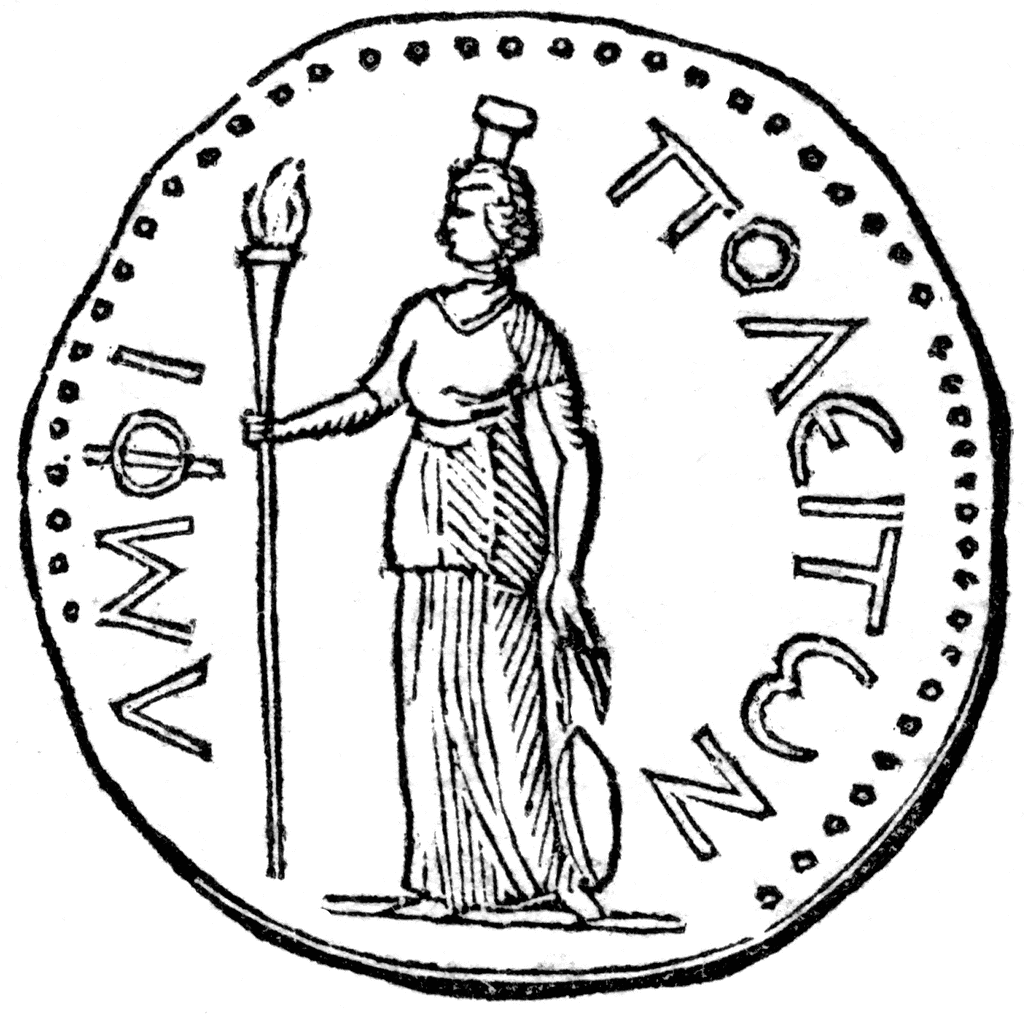
\includegraphics[width=1cm]{TIKZ_SZ/Moneda}};
\draw[>=stealth,->,thick] (-.3,-.35)--(-.75,.45);
\draw (-.525,0) node[left]{\small $\pi_1$};
\draw[>=stealth,->,thick] (-.2,-.35)--(.3,.45);
\draw (.05,0) node[right]{\small $\pi_2 = 1-\pi_1$};
\end{scope}
%
\draw (1.25,-2.25) node{(a)};
\draw (8.25,-2.25) node{(b)};
\end{tikzpicture}